\documentclass[11pt,a4paper]{article}
\usepackage[english]{babel}
\usepackage{graphicx}
\usepackage{epstopdf}
\usepackage{amsmath}
\usepackage{amssymb}
\usepackage{fixltx2e}
%\usepackage[numbered]{mcode}
\usepackage{listings}
\usepackage[margin=1in]{geometry}
\usepackage[parfill]{parskip}
\usepackage{float} %Allow H in figures to fix position with position in text

\newcommand{\mat}[1]{\begin{bmatrix}#1\end{bmatrix}}

\begin{document}

\noindent
\begin{center}
\includegraphics[width=\columnwidth]{tudelftlogo.eps} \\

EE3P11 Electromagnetics\\
\begin{LARGE}
\textbf{Practicum Session 1 \\ Transmission Lines} \\[0.3cm]
\end{LARGE}
\today \\[.2cm]
\begin{tabular}{l l}
Dani\"el Booms & 4284216 \\
Piet De Vaere & 4304241 \\
Nicolaas du Plessis & 4203933 \\
Job van Staveren & 4317386

\end{tabular}
\end{center}



%\begin{abstract}

%\end{abstract}
%\newpage


\subsection*{Introduction}
The first session the EE3P11 EM practicum consists of two parts in which experiments are done with a transmission line. In the first part, the transmission line is considered in the frequency domain. The voltage-standing-wave ratio (VSWR) will be determined for several loads to a source, interconnected by a waveguide. In the second part the transmission lines are considered in the time domain. Reflections due to several loads will be measured. The propagation speed, as well as the relative permittivity, will be estimated for a coaxial cable.

\section{Transmission Lines In Frequency Domain}

\subsection{Experimental Set-up}
%Add pictures of instruction guide
For the first experiment a RF signal source with a frequency $f$ of 9.4756 GHz was used. This signal was modulated with a 1 kHz square wave produced by a waveform generator. The modulated RF signal was sent into a rectangular waveguide. This waveguide contained a slotted line over which a detector could be moved. The detector was connected to an oscilloscope and a digital voltmeter. The reason for modulating the RF source is so that the oscillscope can display the amplitude of the RF signal, as the 1 kHz square wave acts as a trigger. The waveguide could be terminated by various loads. A picture of the set-up can be seen in figure \ref{fig:opstelling1} and a schematic drawing in figure \ref{fig:opstelling1schema}.

\begin{figure}[H]
\centering
\includegraphics[scale=1]{opstelling1.png}
\label{fig:opstelling1}
\caption{Set-up of the first experiment, copied from [3]}
\end{figure}

\begin{figure}[H]
\centering
\includegraphics[scale=1]{opstelling1schema.png}
\label{fig:opstelling1schema}
\caption{Schematic drawing of the set-up of the first experiment, copied from [3]}
\end{figure}

\subsection{Wavelength and Phase velocity}
The wavelength inside the waveguide was measured by moving the detector over the slotted line. Inside the waveguide the signal forms a standing wave, the amplitude of which has sharp minima. By moving the detector from one minimum to another and measuring the distance, the wavelength can be obtained. The distance between two successive minima is half the wavelength. When measuring the wavelength the waveguide was terminated by a 55 mm short circuit. The first minimum measured was at a position of 9.22 cm, the second at 11.39 cm, and the third at 13.61 cm. The wavelength $\lambda$ was therefore 4.39 cm.\\
The phase velocity $v_{p}$ is simply $\lambda \cdot f = 416\cdot 10^{6} \mathrm{ms^{-1}}$. This velocity is higher than the speed of light in vacuum, but this is not a problem as the phase velocity is not the propagation velocity. 

While the phase velocity represents the velocity of a single frequency component of the wave, it does not take into account the individual propagation delays of each component between the two points. Therefore, the phase velocity is more like two events happening consecutively in time, at different locations. As these two points can happen very close together in time, but far apart in distance, this apparent velocity of the phase exceeded the speed of light. Due to these separated occurrence, no information can be transmitted at such speeds, making the phase velocity an essentially useless observation that gives no usable information on the compound waveform.

\subsection{VSWR for various loads}
The waveguide was terminated by five different loads. For all of these loads the maximum and minimum amplitude of the standing wave were measured. From this the VSWR, the reflection coefficient $\Gamma$, and the power delivered to the load $P_{Load}$ were calculated. All this data can be seen in table \ref{tab:LoadData}.\\
The VSWR can be calculated using:
\begin{equation}
\label{eq:VSWR}
VSWR = \frac{|V_{max}|}{|V_{min}|}
\end{equation}
The reflection coefficient can by calculated as:
\begin{equation}
\label{eq:Gamma}
|\Gamma| = \frac{VSWR - 1}{VSWR + 1}
\end{equation}
The power delivered to the load is:
\begin{equation}
\label{eq:PLoad}
P_{Load}=\frac{1}{2}|V_{in}|^{2}Re|\frac{1}{Z_in}|
\end{equation}
where $Z_{in}$ is the input impedance and equals: 
\begin{equation}
\label{eq:Zin}
Z_{in}=Z_{0}\frac{1+\Gamma e^{-j2\beta l}}{1-\Gamma e^{-j2\beta l}}
\end{equation}
with $\beta = \frac{2\pi}{\lambda}$, and $l$ the length of the waveguide from the position of measurement to the load. The characteristic impedance was unknown, but it can easily be calculated when the the reflection coefficient of a known impedance can be determined.
\begin{equation}
\label{eq:Z0}
Z_{0}= Z_{Load}\frac{1-\Gamma}{1+\Gamma}
\end{equation}
In case of the horn antenna the impedance of the load is the characteristic impedance of air, 377$\Omega$. Therefore, with the data from table \ref{tab:LoadData} and equation \ref{eq:Z0} the characteristic impedance of the waveguide could be calculated as $Z_{0}=302\Omega$\\
Because the length of the waveguide was not measured, input impedance could not be calculated, and therefore the power delivered to the load could not be calculated except for the trivial cases. During the experiments the theory was not yet fully understood, and it was forgotten to measure the length of the waveguide.

%table to be used for the first exercises
\begin{table}[h]
\centering
\caption{$\rho, \Gamma$, and $P_{Load}$ for various loads}
\label{tab:LoadData}
\begin{tabular}{|l|l|l|l|l|l|}
\hline
Load                   & $E_{min}$ & $E_{max}$ & VSWR     & $|\Gamma|$ & $P_{Load}$  \\ \hline
a) Open Waveguide      & 26.5mV    & 56.9mV    & 2.15     & 0.37       & unknown            \\ \hline
b) Short Circuit 33 mm & 76.6mV    & 0mV       & $\infty$ & 1.00       & 0           \\ \hline
b) Short Circuit 55 mm & 79.6mV    & 0mV       & $\infty$ & 1.00       & 0           \\ \hline
c) Matched Load        & 41.7mV    & 46.5mV    & 1.12     & 0.057      & unknown            \\ \hline
d) Horn Antenna        & 39.3mV    & 49.0mV    & 1.25     & 0.11       & unknown            \\ \hline
\end{tabular}
\end{table}

\subsection{Standing wave patterns for Short circuits}
The positions of the nodes, i.e. the minima in amplitude, of the standing waves inside the waveguide was measured for both the 33 mm and the 55 mm short circuit. For the 33 mm short circuit, the measured nodes were located at 9.22 cm, 11.39 cm, and 13.61 cm. For the 55 mm short circuit, these were observed at 9.21 cm, 11.42 cm, and 13.60 cm.\\
Generally the position of the nodes shift with a change in length of the short circuit, but the difference in length between the 33 mm and 55 mm short circuit is precisely half of the wavelength. Therefore the nodes are at the same position.

\subsection{Phase velocity for the X-band}
%First additional task
When an EM wave travels in a waveguide, the wavelength is not the same as it is in free space. In the assignment the wavelength inside the waveguide is defined as 
\begin{equation}
\lambda_w=\frac{\lambda_0}{\sqrt{1-(\frac{\lambda_0}{2a})^2}}
\label{phase_velocity}
\end{equation}
with $\lambda_0=\frac{c_0}{f}$ and $c_0$ the speed of light and $f$ the frequency. $a$ is the length of the waveguide, which is 22.86mm.\\
For the phase velocity we now have 
\begin{equation}
v_p=\lambda f = \frac{\lambda_0}{\sqrt{1-(\frac{\lambda_0}{2a})^2}} \cdot f = \frac{c_0}{\sqrt{1-(\frac{\lambda_0}{2a})^2}}
\end{equation}

Figure \ref{v_phase} shows the phase velocity $v_p$ for frequencies in the range of 8-12GHz. From the measurements, a wavelength $\lambda=4.44cm$ was found. Hence the phase velocity equals $v_p=\lambda \cdot f=0.044\cdot9.475\cdot 10^9=4.2\cdot10^8 m/s$.\\

\begin{figure}[H]
\begin{center}
\includegraphics[scale=0.7]{phase_velocity.eps}
\caption{Theoretical phase velocity}
\label{v_phase}
\end{center}
\end{figure}

Since this velocity is an apparent velocity [2] it can travel faster than the speed of light, whereas the EM wave can not. 

\subsection{Additional parameters of waveguide and loads}
If the positions of the nodes for the various loads would have been measured, the impedances of the loads could have been calculated. Since the reflection coeffici\"ent is determined for each load, as well as the impedance $Z_0$ of the waveguide, the load impedance $Z_l$ can be determined.\\
\\
In [2] the phase velocity is defined as
\begin{equation}
v_p=\frac{v}{\sin(\theta)}
\end{equation}
where $v$ is the wave velocity and $\theta$ is the angle the wave makes with the normal to the waveguide surface. Hence if $\theta$ decreases, the phase velocity grows and eventually approaches infinity if $\theta \rightarrow \frac{\pi}{2}$. The same occurs if $\lambda_0=2a$ in equation \ref{phase_velocity}.
Since the phase velocity and the velocity of the wave in free space are know, the angle $\theta$ in equation \ref{phase_velocity} can be determined. This angle equals $\arcsin(\frac{v}{v_p})\approx\frac{\pi}{4}$.

\section{Transmission Lines In Time Domain}

\subsection{Part 1: Time Domain Reflectometry}
\subsubsection{Experimental Set-up}
For this part of the assignment, the setup in Figure \ref{fig:opstelling2a} is used.
A pulse generator injects a sharp pulse into a transmission line ($Z_0 = 50 \ \Omega$),
and the resulting voltage at the input of the transmission line is measured in the time domain.
Assuming the pulse is sufficiently short, this results in a voltage versus time plot,
where the applied pulse and its reflection are clearly distinguishable from each other.

This experiment was performed three times, where the transmission line was kept constant, while different termination loads were used.
The three used loads were:

\begin{itemize}
\item A short circuit
\item A matched load
\item An unknown load
\end{itemize}

\begin{figure}
\includegraphics[scale=1]{opstelling2a.png}
\caption{Setup used for the time domain reflectometry, copied from [3]}\label{fig:opstelling2a}
\end{figure}

\subsubsection{Measurement results and calculations}
The measurements results are shown in Figure \ref{fig:part2aResults}.

\begin{figure}
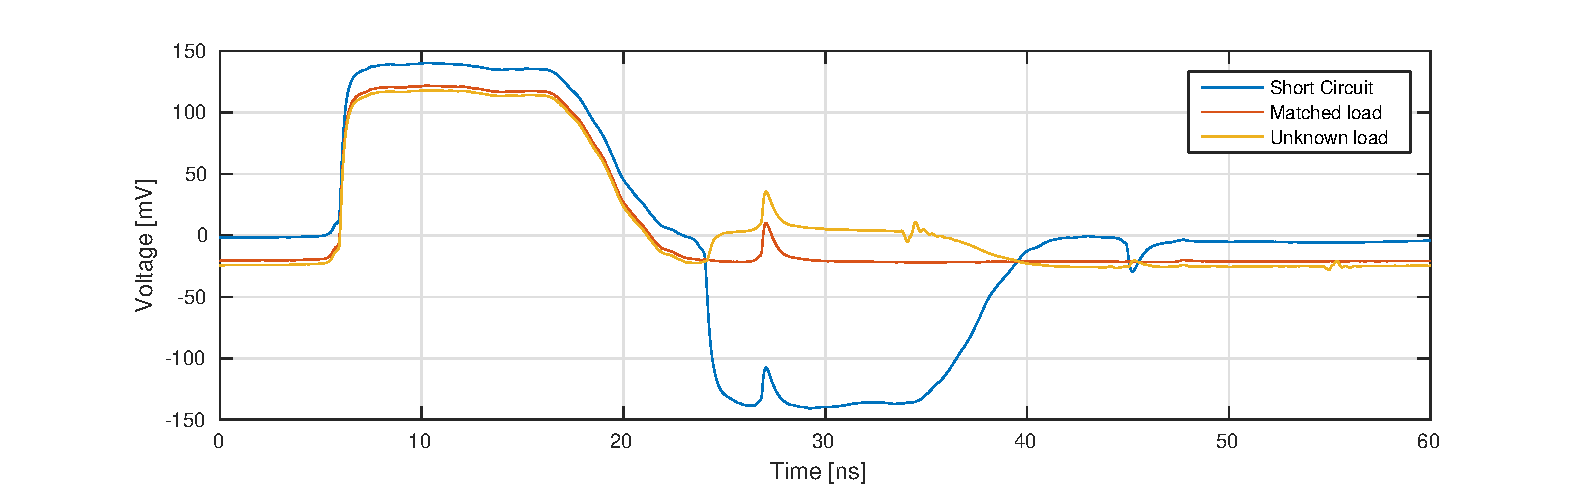
\includegraphics[width=\textwidth]{assignment2aResults.eps}
\caption{The measurement results of inserting a sharp pulse into a transmission line with different terminators.}\label{fig:part2aResults}
\end{figure}

From transmission line theory [2] it is known that the reflection coefficient $\Gamma$ can be calculated as:
\begin{equation} \label{eq:reflectionCoeficient}
\Gamma = \frac{Z_L - Z_0}{Z_L + Z_0}
\end{equation}

Where $Z_L$ is the impedance of the load, and $Z_0$ is the characteristic impedance of the line. Furthermore, the height of the reflected pulse is given by:
\begin{equation}\label{eq:amplitudeReflected}
V^r = \Gamma \cdot V^i
\end{equation}
Where  $V^i$ and $V^r$ are the amplitudes of the incident and reflected pulse, respectively.

These equations will now be evaluated for the two known loads, and the result compared to measured value.

\begin{description}


\item[Short Circuit] Applying Equation \ref{eq:reflectionCoeficient} to a short circuited ($Z_L$ = 0) line predicts a reflection co\"eficient of $\Gamma = -1$.
The measurement results in Figure \ref {fig:part2aResults} show that the amplitude of the incident peak $V^i$ is approximately 140 mV, and that the amplitude of the reflected peak $V^r$ is approximately -140 mV. This is the same value as was predicted by Equation \ref{eq:amplitudeReflected}.

\item[Matched load] Applying Equation \ref{eq:reflectionCoeficient} to a matched ($Z_L$ = $Z_0$) line predicts a reflection co\"eficient of $\Gamma = 0$.
The measurement results in Figure \ref {fig:part2aResults} show the that the amplitude of the incident peak $V^i$ is approximately 140 mV, and that no reflected peak is measured $V^r = 0$ V. This is the same value as was predicted by Equation \ref{eq:amplitudeReflected}.
\end{description}

If $V^i$, $V^r$ and $Z_0$ are known, Equations \ref{eq:reflectionCoeficient} and \ref{eq:amplitudeReflected} can be used to determine $Z_L$. This will now be done for the unknown load.
Figure \ref {fig:part2aResults} shows $V^i \approx$ 140 mV, and that $V^r \approx$ 28 mV. Using Equation \ref{eq:amplitudeReflected}, it is calculated that $\Gamma\approx 0.2$. Using Equation \ref{eq:reflectionCoeficient} and knowing that $Z_0 = 50 \ \Omega$, it is calculated that:
\begin{equation}
Z_L = - Z_0 \cdot \frac{\Gamma + 1}{\Gamma - 1} \approx - 50 \ \Omega \cdot \frac{0.2 + 1}{0.2 -1} = 75 \ \Omega
\end{equation}

Because only the difference in amplitude --- and not in phase --- is known, it is assumed that the reflection co\"eficient and load impedance are real.
This is probably a good approximation.

Note that while in the frequency domain a virtually infinite sinusoidal signal was used as input signal. This signal consisted of a single frequency.
Consequently, the resulting interference patterns (amplitude versus position) where measured.
On the other hand, in the time domain a single, sharp, narrow pulse was used as input signal. In the ideal case, this signal consists of \emph{all} frequencies.
Consequently, the amplitude of the waves was measured versus time.

\subsection{Part 2: Dielectric In Coaxial Cable}
\subsubsection{Experimental Set-up}
For the second part of the second assignment, the measurement set-up is modified. The new set-up is shown in Figure \ref{fig:opstelling2b}. Instead of measuring the voltage at the beginning of the cable, the voltage at the \emph{end} of the cable is measured. This allows to measure the time it takes a pulse to travel through the cable.

Two measurements are performed using this set-up:
\begin{itemize}
\item First, a calibration cable is connected measurement system.
\item Next, an extra piece of cable --- under investigation --- is connected between the calibration cable and the sampling unit. The length of this cable under test is $x$ = 2.0 m.
\end{itemize}

By comparing the two measurements, it will be possible to calculate the wave propagation speed in the cable under test.

\begin{figure}
\includegraphics[scale=1]{opstelling2b.png}
\caption{Setup used for the estimation of propagation speed and relative permitivity of a cable, copied from [3]}\label{fig:opstelling2b}
\end{figure}

\subsubsection{Measurement results and calculations}
The measurements results are shown in Figure \ref{fig:part2bResults}. The time difference between the two rising edges is $\Delta t = $ 8.8 ns.

Assuming that waves propagate through the line with a constant speed, the propagation speed $c$ becomes:
\begin{equation}
c = \frac{x}{\Delta t} = \frac{2.0 \text{ m}}{8.8 \text{ ns}} = 2.2 \cdot{10^8} \ \frac{\text{m}}{\text{s}}
\end{equation}

Furthermore, it is know from transmission line theory [2] that 
\begin{equation}\label{eq:propagationspeed}
c = (\mu\epsilon)^{-1} = (\mu_0\mu_r\epsilon_0\epsilon_r)^{-1} = c_0(\mu_r\epsilon_r)^{-1}
\end{equation}

where $\mu$, $\mu_r$ and  $\mu_0$ are the permeability of the medium, the relative permeability of the medium and the  permeability of vacuum, respectively. $\epsilon$, $\epsilon_r$ and  $\epsilon_0$ are the permittivity of the medium, the relative permittivity of the medium and the  permittivity of vacuum, respectively. $c_0$ is the wave propagation speed in vacuum.

Using Equation \ref{eq:propagationspeed}, and assuming $\mu_r$ = 1, the relative permittivity of the dielectric in the cable can be calculated as:
\begin{equation}
\sqrt{\epsilon_r\mu_r} = \frac{c_0}{c} \Leftrightarrow
\sqrt{\epsilon_r} = \frac{c_0}{c} \Leftrightarrow
\epsilon_r = \left(\frac{c_0}{c}\right)^2 = \left(\frac{3 \cdot 10^8 \text{ m/s}}{2.2 \cdot 10^8 \text{ m/s}}\right)^2 \approx 1.86
\end{equation}


\begin{figure}
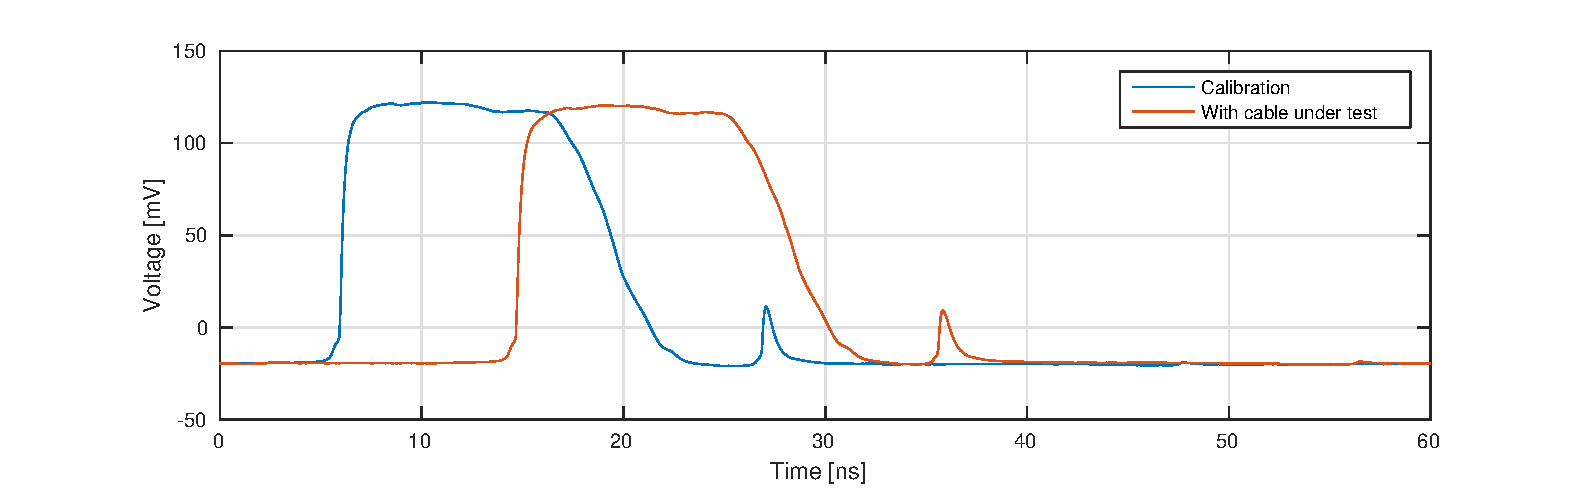
\includegraphics[width=\textwidth]{assignment2bResults.eps}
\caption{The mesurement results when applying a sharp pulse to the beginning of a transmission line, and measuring the voltage at the output}\label{fig:part2bResults}
\end{figure}

\section{Conclusion}
In the first session of the EE3P11 practicum transmission lines where investigated both in the time and frequency domain.

In the frequency domain, a sinusoidal signal was used as input, and the interference patterns where measured.
With this information the VSWR and reflection co\"eficient were calculated for different loads. These results are shown in Table \ref{tab:LoadData}.
Due to missing measurement data, the load impedances could not be calculated.
The phase velocity in the transmission line was determined to be $v_p = 416 \cdot 10^6$ m/s.

In the time domain, a single widebanded pulse was used as input, and the resulting wave amplitude versus time was measured.
Two experiments were performed.
Firstly, the value of an unknown termination load ($Z_L = 75 \ \Omega$) was determined.
Next, the wave propagation speed ($c = 2.2 \cdot 10^8$ m/s) and relative permittivity ($\epsilon_r = 1.86$) of a coaxial cable with known length were calculated.

\section{References}
[1]  LaTeX tables generated using http://www.tablesgenerator.com/\\
{[2]} A.L. Lance, \textit{Introduction To Microwave Theory And Measurements}, New York: McGraw-Hill, 1964.\\
{[3]} \textit{EE3P11 - EM Practicum, 2015-2016 Q3}, TU Delft, Delft, Netherlands, 2016.


\end{document}
